\documentclass[12pt]{article}
\usepackage[utf8]{inputenc}
\usepackage[english, russian]{babel}
\usepackage{graphicx, float, multicol, hyperref, pgfplots}

\title{Определение модуля Юнга на основе исследования деформаций растяжения и изгиба}
\author{Балдин Виктор}

\begin{document}
    \maketitle

    \section{Aннотация}
    \par \textbf{Цель работы:} экспериментально получить зависимость между напряжением и деформацией
    для двух простейших напряженных состояний упругих тел: одностороннего сжатия и чистого изгиба;
    по результатам эксперимента вычислить модул Юнга.\\
    \par \textbf{В работе используются:} в первой части - прибор Лермантова, проволока
    из исследуемого материала,
     зрительная трубка со шкалой,
    набор грузов, микрометр, рулетка;  во второй части - стойка для изгибания балки, индикатор для
    измерения величин прогиба,
набор исследуемых стержней, грузы, линейка, штангенциркуль.

    \section{Определение модуля Юнга по измерениям растяжения проволоки}
    \subsection{Теоретические сведения}
    Растяжение проволоки соответствует напряженному состоянию вдоль одной оси, которое описывается формулой:
\begin{equation}
    \frac{F}{S} = E \frac{\Delta l}{l}
    \label{lermantov}
\end{equation}
    Эту формулу можно переписать также в следующем виде:
    \begin{equation}
        F = k\Delta l,
    \end{equation}
    где $k = ES / l$ -- жесткость проволоки.
    Измерения производятся на установке Лермантова.
    Направим зрительную трубку на зеркальце.
    Выведем формулу для расчета растяжения длины проволоки по показаниям шкалы
    прибора (см. рис. 1).
    Так как мы считаем проволоку слабо растяжимой, справедлива оценка $\Delta l \ll r$, где
    $r$ -- длина рычага. С учетом этого, угол наклона зеркальца к горизонтали можно
    найти как $\alpha = \Delta l/r$. С другой стороны, из соображений геометрической оптики
    угол $\alpha$ можно найти как угол между продолжениями соответствующих лучей:
    \begin{equation}
        \alpha = \frac{n\Delta h}{2h},
    \end{equation}
    где $\Delta h$ -- цена деления шкалы, $n$ -- число делений, $h$ -- расстояние от шкалы до
    зеркальца.
    \par Таким образом, удлинение проволоки можно выразить как:
    \begin{equation}
        \Delta l = n\Delta h\frac{r}{2h}
        \label{dlina}
    \end{equation}

    \subsection{Методика измерений}
    \par Для определения модуля Юнга используется прибор Лермонтова,
    схема которого изображена на рис. 1. Верхний конец проволоки П, изготовленной
    из исследуемого материала, прикреплен к консоли К, а
    нижний -- к цилиндру, которым оканчивается шарнирный кронштейн
    Ш. На этот же цилиндр опирается рычаг $r$, связанный с зеркальцем
    3. Таким образом, удлинение проволоки можно измерить по углу
    поворота зеркальца.\\
    \par Натяжение проволоки можно менять, перекладывая грузы с
    площадки М на площадку О и наоборот. Такая система позволяет
    исключить влияние деформации кронштейна К на точность измерений, так
    как нагрузка на нем все время остается постоянной.

    \begin{figure}[H]
        \centering
        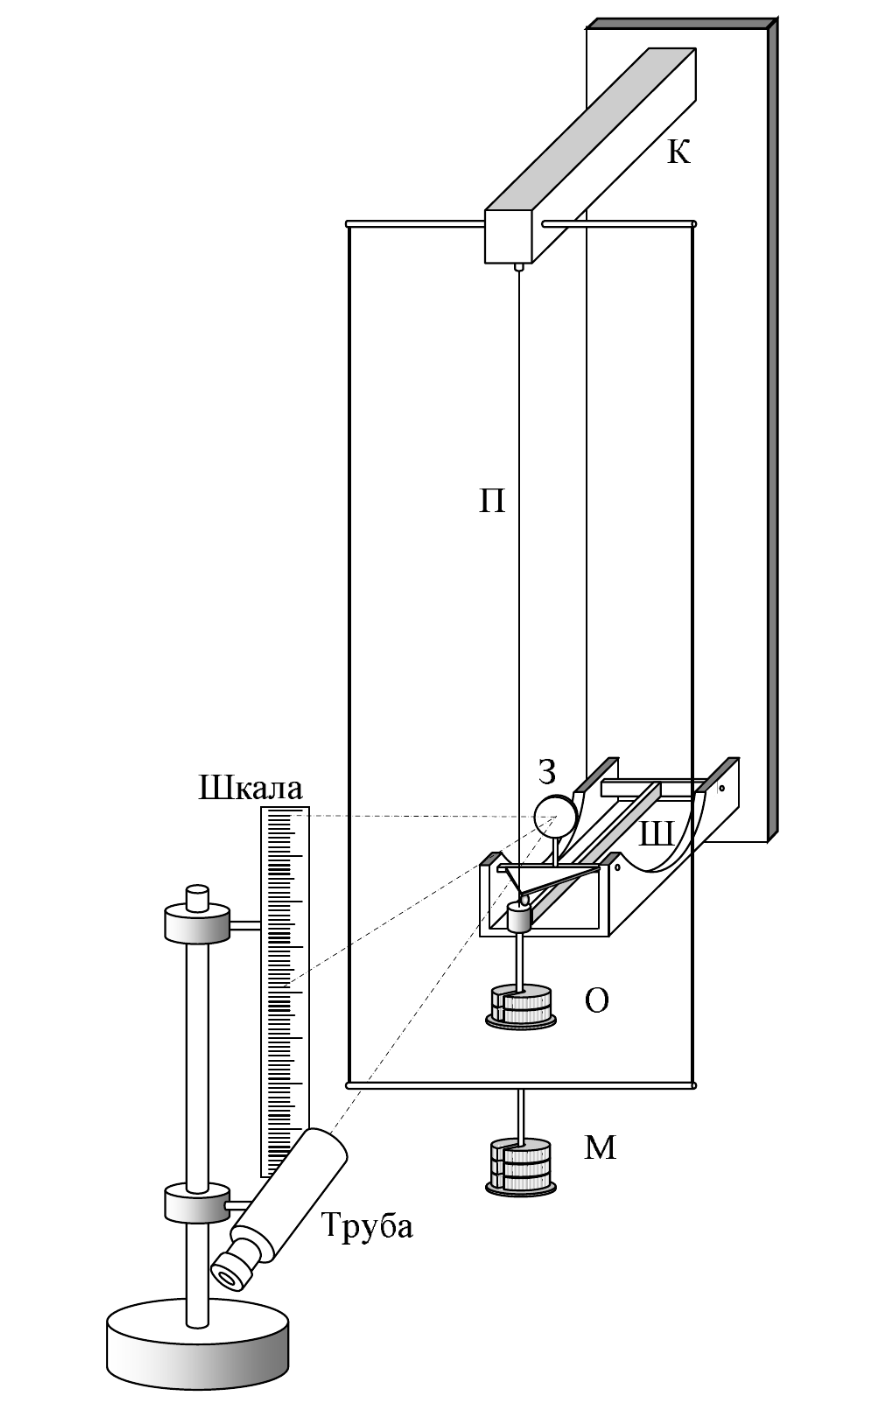
\includegraphics[scale = 0.3]{pictures/lermantov.png}
        \caption{Прибор Лермантова}
    \end{figure}

    \subsection{Используемое оборудование}
    Рулетка, микрометр для измерения параметров установки (погрешность
    $0.5\pm10^{-5}$ м).
    ; прибор Лермантова, проволока
    (разрушающее напряжение 900 Н/мм$^2$).
    \par Диаметр проволоки входит в формулы во 2-й степени, значит,
    он потенциально имеет большее влияние на итоговый результат.
    Однако это нивелируется высокой точностью измерения при помощи
    микрометра.

    % \subsection{Результаты измерений и обработка данных}
    \section{Определение модуля Юнга по измерениям изгиба балки}
    \subsection{Теоретические сведения}
    Модуль Юнга материала стержня $E$ связан с величиной
    прогиба $y_{max}$ как:
    \begin{equation}\label{balka}
        E=\frac{Pl^3}{4ab^3y_{max}}
    \end{equation}
    где $P$ - нагрузка на стержень, $l$ - расстояние меду точками опоры,
    $a$ - ширина балки, $b$ - высота балки.

    \subsection{Экспериментальная установка}
    \par Экспериментальная установка состоит из прочной стойки с
    опорными призмами А и Б (рис. 2). На ребра призм опирается исследуемый
    стержень В. В середине стержня на призме Д подвешена площадка
    П с грузами. Измерять величину
    прогиба можно с помощью индикатора И, укрепляемого
    на отдельной штанге. Полный оборот большой
    стрелки индикатора соответствует 1 мм и одному делению малого циферблата.
    \begin{figure}[H]
        \centering
        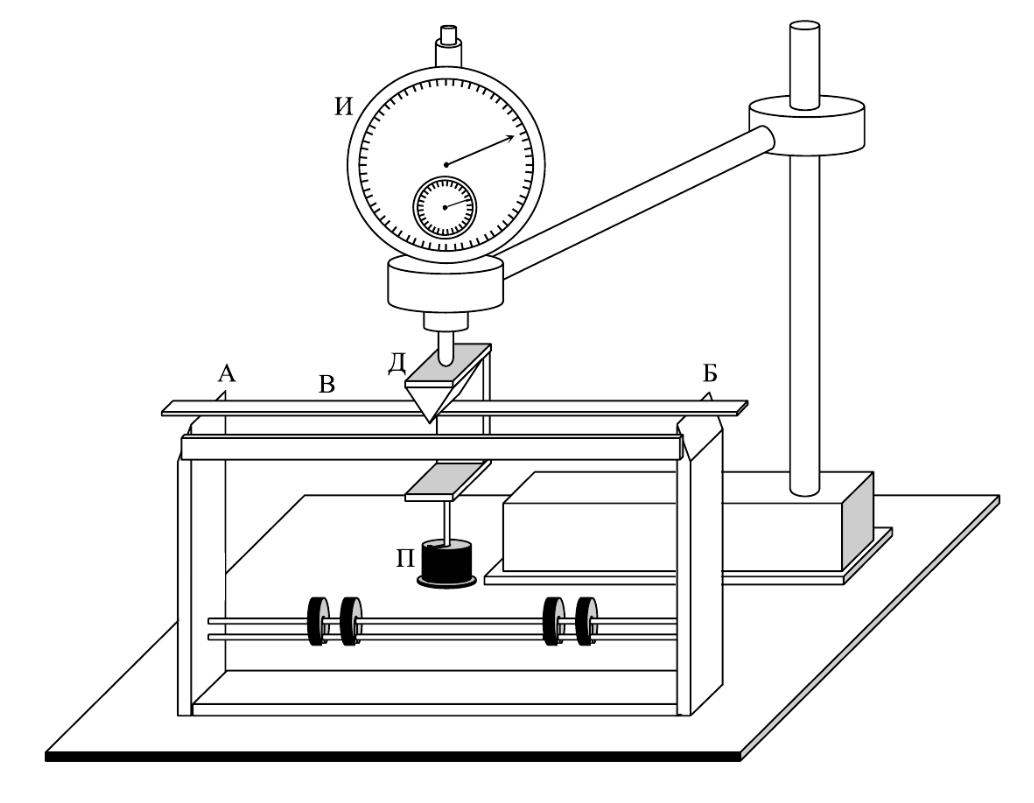
\includegraphics[scale = 0.25]{pictures/balka.png}
        \caption{Схема установки для измерения модуля Юнга}
    \end{figure}

    \subsection{Используемое оборудование}
    Линейка, штангенциркуль для измерения параметров установки;
    индикатор для измерения стрелы прогиба.
    \par Для уменьшения погрешности вследствие прогиба стола
    при изменении нагрузки на стержень, грузы перед началом эксперимента
    лучше расположить на рейке над нижней полкой опорной стойки.

\end{document}
